\chapter{Evaluation}
\thispagestyle{fancy}
\label{chap:Evaluation}

\noindent
In diesem Kapitel werden die zuvor konzipierten Experimente umfangreich evaluiert. Dies geschieht einerseits auf Basis der ausgewählten Metriken, andererseits in Form einer qualitativen Analyse der aus den Anhängen A und B generierten Zusammenfassungen.


\section{Automatische Auswertung}
\noindent
Das erste Experiment sieht die Reproduktion des \ac{SOTA} vor und basiert konsequenterweise auf den englischsprachigen Daten ($K_{eng}$). Dabei werden in \autoref{table:ExpEnScores} die \ac{ROUGE}-Scores von \ac{BERT} und \ac{XLM-R} miteinander verglichen.\\

\begin{table}[htb]
\centering
\begin{tabular}{ | p{2.5cm} | p{2.5cm} | p{2.5cm} | p{2.5cm} | }
\hline
\textbf{Modell} & \textbf{R-Recall} & \textbf{R-Precision} & \textbf{R-Measure} \\
\hline
BERT & 15.78 & 10.25 & 12.11 \\
\hline
XLM-R & 11.76 & 8.89 & 9.88 \\
\hline
\end{tabular}
\caption{SOTA-Reproduktion im Modellvergleich.}
\label{table:ExpEnScores}
\end{table}

\begin{figure}[h]
  \centering
  \fbox{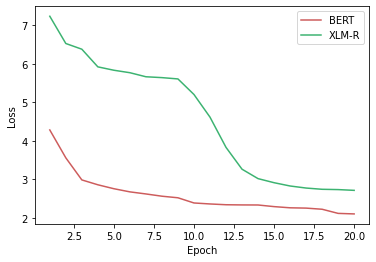
\includegraphics[width=0.6\linewidth]{./source/images/lossenglish.png}}
  \caption{Loss in der SOTA-Reproduktion im Modellvergleich.}
  \label{pic:ExpEnLoss}
\end{figure}

\noindent
\ac{BERT} ist demnach unter Akzeptanz womöglich unbekannter Nebenbedingungen \ac{SOTA}-konform. \ac{XLM-R} hingegen bleibt weit zurück und bedarf aufgrund der komplexen Architektur einem noch umfangreicheren Fine-Tuning. Die Lernfortschritte sind anhand der Fehlerentwicklung in \autoref{pic:ExpEnLoss} visualisiert. Hierbei ist der Rückstand von \ac{XLM-R} nachvollziehbar.\\

\noindent
Im zweiten Experiment ist die Adaption der Modelle auf die deutsche Sprache vorgesehen. Hierfür kommen konsequenterweise ausschließlich die deutschsprachigen Daten ($K_{wik} \cup K_{nws} \cup K_{mls}$) zum Einsatz. Die \ac{ROUGE}-Scores der zwei zu vergleichenden Modelle sind \autoref{table:ExpDeScores} zu entnehmen. Es ist zu erkennen, dass \ac{BERT} wertmäßig in Englisch genauso gut wie in Deutsch ist. Der \ac{SOTA} wird indes unter Akzeptanz eines gewissen Rauschens von beiden Modellen erreicht. Die Lernfortschritte sind in bekannter Weise in \autoref{pic:ExpDeLoss} visualisiert. Hier ist zudem die Assimilation beider Modelle nachvollziehbar.\\

\begin{table}[htb]
\centering
\begin{tabular}{ | p{2.5cm} | p{2.5cm} | p{2.5cm} | p{2.5cm} | }
\hline
\textbf{Modell} & \textbf{R-Recall} & \textbf{R-Precision} & \textbf{R-Measure} \\
\hline
BERT & 15.93 & 10.52 & 11.97 \\
\hline
XLM-R & 15.93 & 10.32 & 11.86 \\
\hline
\end{tabular}
\caption{Adaption auf deutschen Daten im Modellvergleich.}
\label{table:ExpDeScores}
\end{table}

\begin{figure}[h]
  \centering
  \fbox{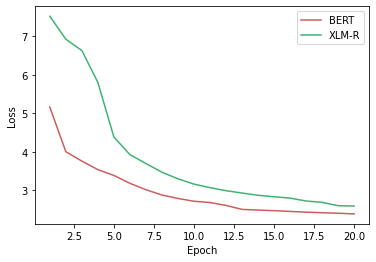
\includegraphics[width=0.6\linewidth]{./source/images/lossgerman.png}}
  \caption{Loss in der Adaption auf deutschen Daten im Modellvergleich.}
  \label{pic:ExpDeLoss}
\end{figure}
\newpage

\noindent
In dritten Experiment wurden alle verfügbaren Daten ($K_{eng} \cup K_{wik} \cup K_{nws} \cup K_{mls}$) genutzt, um beide Modelle dem Fine-Tuning zu unterziehen. \ac{BART} wird indes aus externer Quelle bezogen. Dabei sind die in \autoref{table:ExpMlScores} dokumentierten \ac{ROUGE}-Scores zu verzeichnen. Es wird ersichtlich, dass sich \ac{BERT} unter multilingualen Trainingsdaten verbessert, \ac{XLM-R} hingegen nicht. In \autoref{pic:ExpMlLoss} wird zudem deutlich, dass \ac{XLM-R} erst spät, dann aber zielgerichtet trainiert. \ac{BART} ist aufgrund des externen Bezugs nicht vertreten, tritt allerdings bezüglich der \ac{ROUGE}-Scores wertmäßig deutlich hervor.\\

\begin{table}[htb]
\centering
\begin{tabular}{ | p{2.5cm} | p{2.5cm} | p{2.5cm} | p{2.5cm} | }
\hline
\textbf{Modell} & \textbf{R-Recall} & \textbf{R-Precision} & \textbf{R-Measure} \\
\hline
BERT & 16.76 & 11.18 & 12.68 \\
\hline
XLM-R & 15.13 & 9.55 & 11.08 \\
\hline
BART & 0.00 & 0.00 & 0.00 \\
\hline
\end{tabular}
\caption{Adaption auf multilingualen Daten im Modellvergleich.}
\label{table:ExpMlScores}
\end{table}

\begin{figure}[h]
  \centering
  \fbox{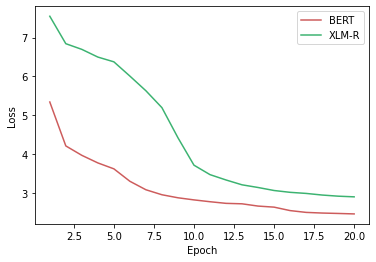
\includegraphics[width=0.6\linewidth]{./source/images/lossmultilingual.png}}
  \caption{Loss in der Adaption auf multilingualen Daten im Modellvergleich.}
  \label{pic:ExpMlLoss}
\end{figure}
\newpage


\section{Qualitative Analyse}
\noindent
Die soeben evaluierten Experimente werden nun ergänzend qualitativ analysiert. Hierfür werden die Modelle aller Experimente sprachabhängig entweder Anhang A oder Anhang B unterzogen, indem die dort enthaltenen mitunter herausfordernden Texte maschinell zusammengefasst und subjektiv bewertet werden. Eine derartige Analyse ist erforderlich, um die Qualität sowie die praktische Eignung der trainierten Modelle vollends beurteilen zu können. Die qualitative Analyse ist außerdem erforderlich, um den teilweise kritisch begutachteten sowie eher statistisch veranlagten \ac{ROUGE}-Score qualitativ einzuordnen. Zudem sei bemerkt, dass die Zusammenfassungen in englischer und deutscher Sprache modellübergreifend den Anhängen C und D zu entnehmen sind.\\

\noindent
Zuerst werden die englischen Modelle miteinander verglichen, namentlich \ac{BERT} und \ac{XLM-R}. Die obige Auswertung hebt hierbei \ac{BERT} als wertmäßig bestes Modell hervor. Die generierten Zusammenfassungen bestätigen diese Aussage aus praktischer Sicht für die getroffene Modellauswahl, obwohl Informationen teilweise leicht fehlerbehaftet sind. Dies wird im Kontext dieser Arbeit als \ac{SOTA}-konform interpretiert. \ac{XLM-R} hingegen ist unbrauchbar, insbesondere wegen der ungenügenden Grammatik und Orthographie. Somit sind auch viele der neu generierten Informationen schlichtweg falsch.\\

\noindent
Gemäß des Vergleichs der deutschen Modelle entspricht \ac{BERT} zwar wertmäßig dem \ac{SOTA}, schneidet jedoch vor allem bei Texten unbekannter Art eher schlecht ab. Dabei wird die Abhängigkeit des Modells von der Beschaffenheit der Trainingsdaten deutlich, insbesondere anhand der Natur der Zusammenfassungen. Hier ist nämlich ein typisches Element der Nachrichtendomäne erkennbar, da anstatt einer konventionellen Zusammenfassung oftmals ein Teaser generiert wird, der den Leser binden und zum Text weiterleiten soll. Dieses Verhalten ist jedoch nicht auf das Modell zurückzuführen, sondern auf die Trainingsdaten, welche größtenteils eben jener Nachrichtendomäne entstammen. Dies unterstreicht insgesamt die Notwendigkeit einer intensiven Datenanalyse. Hinsichtlich eines praktischen Einsatzes ist also stets ein anforderungsgerechter Korpus zu formieren. Zudem ist der Einfluss des vortrainierten Modells bemerkbar, beispielsweise im Text über das Finale der WM 2014. Hier wird im originalen Text von Jogi Löw geschrieben, in der Zusammenfassung hingegen von Jürgen Klopp. Letzterer wurde zuvor jedoch nie erwähnt. Dies kann mit der geringen Distanz beider Personen im Vektorraum erklärt werden und ist somit zwar sachlogisch falsch, mathematisch jedoch nachvollziehbar. Dies tritt in ähnlicher Weise auch in den anderen Zusammenfassungen auf. Ein Fine-Tuning mit sehr viel mehr Trainingsdaten verspricht dieses Rauschen hinreichend zu minimieren.
\newpage

\noindent
Die \ac{ROUGE}-Scores der deutschen \ac{XLM-R} lassen eine Verbesserung gegenüber der englischen \ac{XLM-R} vermuten. Dies lässt sich mithilfe der qualitativen Analyse bestätigen. Die zuvor ungenügende Grammatik und Orthographie ist nun korrekt erlernt. Gegenüber dem deutschen \ac{BERT} sind die inhaltlichen Schwächen zwar reduziert, jedoch nicht vollumfänglich beseitigt. Ansonsten ist erwartungsgemäß erneut das lockende Element aus der Nachrichtendomäne erkennbar. Dies wird bekanntermaßen von den Trainingsdaten bewirkt, weshalb dieses Verhalten wohl modellübergreifend auftritt.\\

\noindent
Auf der multilingualen Datengrundlage verbessert sich \ac{BERT} wertmäßig. Subjektiv verbessert er sich in Englisch nun bis zur praktischen Eignung, in Deutsch jedoch nicht. In deutscher Sprache ist ein Overfitting in Form von auswendig gelernten Sätzen erkennbar. \ac{XLM-R} ...\\ % TODO: ...

\noindent
\ac{BART} weist aufgrund der identischen Datengrundlage ein ähnliches Verhalten wie \ac{BERT} und \ac{XLM-R} auf, scheint jedoch robuster zu sein und insgesamt weniger Fehler zu machen. Dennoch sind auch hier inhaltliche Mängel sowie erstmalig auch englische Wörter in einer deutschen Zusammenfassung zu verzeichnen. Entgegen obig formulierter Erwartung scheint \ac{BART} dem lockenden Element der Nachrichtendomäne nicht nachzukommen. \ac{BART} ist für die \ac{ATS} in englischer Sprache das Modell der Wahl, in deutscher Sprache vermutlich nur mit einem hinreichenden Fine-Tuning. \ac{BERT} ist wertmäßig und subjektiv wieder Erwarten nur leicht unterlegen.\\

\noindent
TODO: ...

% TODO: Bewährtes Modell auswählen, zu Optimierungszwecken weiter experimentieren

% TODO: Übersetzungen, Data Augmentation und Sliding Window Approach in den Ausblick verschieben, Texte untenstehend sukzessive geraderücken und komplettieren, profitieren multilinguale Modelle von dem verborgenen Strukturen anderer Sprachen?

\noindent
Trotz der monolingualen Fortschritte wird \ac{GBERT} zunächst durch \ac{XLM-R} und anschließend durch \ac{BART} ersetzt, um sich weiterhin geeigneten Ergebnissen zu nähern und multilinguale Modelle zu erproben. Der Tokenizer wird ebenfalls entsprechend ausgetauscht. Es entstehen die folgenden \ac{ROUGE}-Scores: R-Recall: 23.02, R-Precision: 13.95, R-Measure: 16.09. Obgleich \ac{XLM-R} bewiesenermaßen verschiedene \ac{NLP}-Aufgaben begünstigt, kann sie in der vorliegenden Konfiguration keine Verbesserung der \ac{ATS} erzielen. Dies basiert nicht nur auf den verringerten \ac{ROUGE}-Scores, sondern auch auf der nachfolgenden exemplarischen Zusammenfassung von Anhang B, welche inhaltlich subjektiv als mangelhaft eingestuft werden kann.\\

\noindent\fbox{%
\parbox{\textwidth}{%
Der 11. Flugtag der Weltturm-Weltmeisterschaft 2001 fand am 11. September 2001 in New York City statt und war das erste Mal in der Geschichte des World Trade Centers. Das National September 11 Memorial and Museum in Manhattan ist ein historischer Gedenkpavillon in Manhattan. Es befindet sich in der Nähe des World Trade Centers in Manhattan.
}%
}\\

% TODO: BART trainieren und kritisieren, evtl. ist GBERT trotzdem besser

\noindent
In der Konsequenz wird \ac{GBERT} für die weiteren Experimente genutzt. Hierbei werden insbesondere die Anteile der jeweiligen Korpora an den Trainings- und Testdaten variiert, um vornehmlich dem Lernen der Textstruktur entgegenzuwirken. Die Konfigurationen sowie entsprechende Ergebnisse sind der Tabelle ? zu entnehmen.\\

% TODO: Tabelle ? nach erfolgten Trainingsschritten erstellen, oben referenzieren und Erkenntnisse beschreiben/ herausstellen, weitere Schritte begründet anschließen, bspw. Data Augmentation, Übersetzung englischsprachiger Korpora, Parts im Example überarbeiten, Experimente im Excel kompaktieren, bspw. letztes Tabellenblatt

\noindent
- Training auf Wiki, Evaluation auf News
  -> Sehr schlecht, strukturerlernend
- Training auf News mit ein bisschen Wiki, Evaluation mit New
   -> Positiver Effekt, aber zu wenig Daten
- Training auf News und 50 Prozent von Wiki, Evaluation mit News
  -> ?
- Training auf übersetztem CNN/ Dailymail, Evaluation mit News
  -> ?

% TODO: Experimente erneut in einer Tabelle zusammenfassen, siehe Tabelle im abstraktiven Ansatz, verschiedene Spalten für verschiedene Parameterkonfigurationen anfügen

% TODO: Sliding-Window-Approach bei zu großen Texten beschreiben und entwickeln, beim Laden der Texte, aber als separate Methode, die auf einzelne Texte anwendbar ist, trotzdem mit Map als Batch-Verarbeitung, über Bool in der Config beim Training auswählbar machen, im Beispiel als Methode einbinden, prinzipiell lange Texte behandeln, ggf. über Konkatenation, mindestens im Ausblick herausstellen

% TODO: Kapitel besser strukturieren (format-technisch, inhaltlich), German Abstractive Summarization lesen und einarbeiten, Beschreibung der Datengrundlage nochmal überprüfen, Lorem ipsum und TODO's in beiden Kapiteln herausarbeiten, Hyperparameteroptimierung auf 10-20 Prozent der Daten vornehmen, Verdichtung der Zusammenfassung verdeutlichen, d.h. Token-Reduktion, zudem die prozentuale Kompressionsrate angeben (75% von 512 auf 128 Token), d.h. mit technischen Anpassungen können auch 5 DIN A4-Seiten um x Prozent verdichtet werden (Wie lang ist der Eingangstext? Wie lang ist der Ausgangstext? Wie geht das Modell mit längeren Texten um?)

% TODO: \cite{YAN19} S. 4 rechts, Herausforderung: Encoder overfitted, Decoder underfitted oder andersherum, wird durch HuggingFace-Framework vorgebeugt, \cite{YAN19} S. 5 oben für Evaluation, Vergleichstabelle der Experimente einbinden und beschreiben, typisches Diagramm zur Visualisierung des Trainingsprozesses anfügen, Verhalten des Modells interpretieren und Anpassungen ableiten, bspw. Exploitation wegen der Struktur der Artikel nochmal aufgreifen, ggf. erst bei der sprachtechnischen Adaption, erwähnen, dass dies als Experiment genügt, sprachtechnische Anpassungen dann erst im nächsten Kapitel, Referenzzusammenfassungen mit ROUGE und BLEU bewerten, um Vergleichswerte nennen zu können, Texte manuell zusammenfassen, um ebenfalls einen Vergleichswert von ROUGE und BLEU zu haben\\

% TODO: Dateien vom Taurus herunterladen und synchronisieren
